\begin{frame}
  \frametitle{Authentification et contrôle d'accès}
  \begin{block}{\textbf{ Sommaire }}
  \begin{itemize}
  \item Les choix
  \item Architecture
  \item Gestion des droits
  \item Les Protocoles
  \item Réalisation
  \end{itemize}
  \end{block}
\end{frame}

\begin{frame}
  \frametitle{Authentification et contrôle d'accès}
  \begin{block}{\textbf{Pourquoi un annuaire ? }}
  \begin{itemize}
  \item Plus consulté que mis à jour
  \item Structure hierachique 
  \end{itemize} 
  \end{block}
\end{frame}

\begin{frame}
  \frametitle{Authentification et contrôle d'accès}
  \begin{block}{\textbf{Pourquoi LDAP ? }}
  \begin{itemize}
  \item Protocole réseau léger
  \item Recherche simple et critérisée
  \item Organisation des résultats
  \item Mécanisme de référencement
  \item Authentification et contrôle d'accès
  \item Haute disponibilité via réplication
  \end{itemize}
  \end{block}
\end{frame}

  \frametitle{Authentification et contrôle d'accès}
  \begin{figure}[htbp]
	  \centering
	  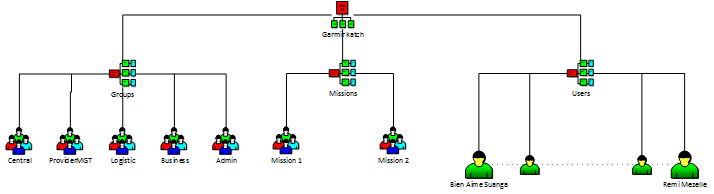
\includegraphics[scale=0.6]{Images/SchemaLDAP.png}
	  \caption{Structure de l'annuaire}
	  \label{SchemaLDAP}
  \end{figure}
 
  \begin{figure}[htbp]
	\centering
	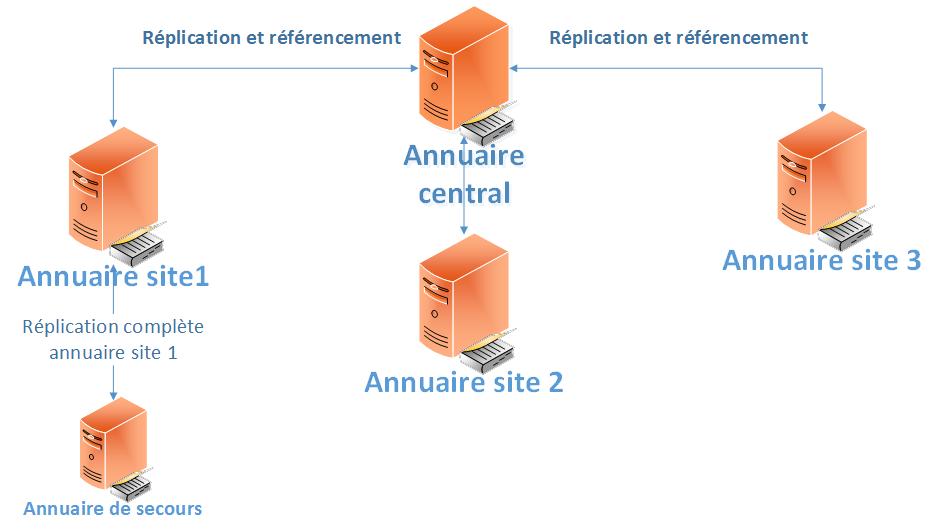
\includegraphics[scale=0.4]{Images/SchemaGlobal.png}
	\caption{Architecture globale}
	\label{SchemaGlobal}
\end{figure}

\begin{figure}[htbp]
	\centering
	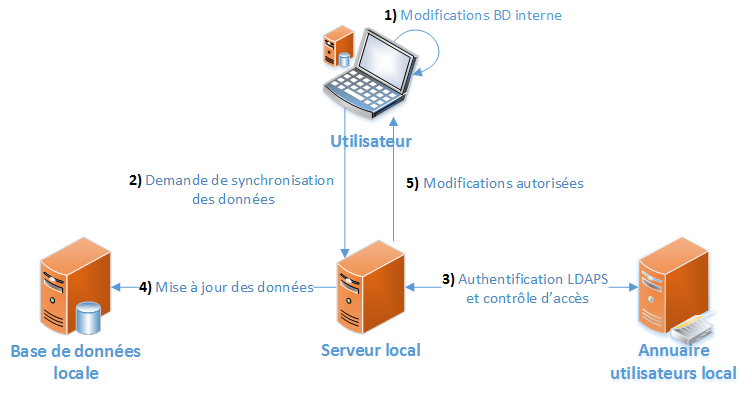
\includegraphics[scale=0.6]{Images/SchemaAuthentification.png}
	\caption{Authentification pour la synchronisation}
	\label{SchemaAuthentification}
\end{figure}

\begin{frame}
  \frametitle{Authentification et contrôle d'accès}
  \begin{block}{\textbf{Droits utilisateurs}}
  \begin{itemize}
  \item Droits pour chaque utilisateur
  \item Droits pour chaque groupe
  \item Autorisations et/ou refus
  \end{itemize}
  \end{block}
\end{frame}

\begin{frame}
  \frametitle{Authentification et contrôle d'accès}
  \begin{block}{\textbf{Gestion des droits}}
  \begin{itemize}
  \item Priorité aux droits directement liés à l'utilisateur 
  \item Priorité aux droits autorisés si l'utilisateur est lié à plusieurs groupes
  \item les droits du groupe
  \end{itemize}
  \end{block}
\end{frame}

\begin{frame}
  \frametitle{Authentification et contrôle d'accès}
  \begin{block}{\textbf{Autres Protocoles connus}}
  \begin{itemize}
  \item RADIUS (Remote Authentication Dial-In User Service)
  \item PAP (Password Authentication Protocol)
  \item MS-CHAP (Microsoft Challenge Handshake Authentication Protocol)
  \item ... 
  \end{itemize}
  \end{block}
%   Utiles si on sait comment se defendre face à une question
%   \begin{block}{\textbf{Quelques normes utiles}}
%   \begin{itemize}
%   \item X500 
%   \item UDDI : Universal Description Discovery and Integration
%   \item TULLEB : Titre Uniforme Labellisé Librement et Édité(Norme destinée aux annuaires publicitaires)
%   \item ... 
%   \end{itemize}
%   \end{block}
\end{frame}

\begin{frame}
  \frametitle{Authentification et contrôle d'accès}
  \begin{block}{\textbf{Travail effectué}}
  \begin{itemize}
  \item Mis en place du serveur 
    \begin{itemize}
    \item Windows
    \item Linux
    \end{itemize}
  \item Ajout d'un schema 
  \item Librairie de consulation via l'outil % à rénomer 
  \end{itemize}
  \end{block}
\end{frame}

\begin{frame}
  \frametitle{Authentification et contrôle d'accès}
  \begin{block}{\textbf{ceux qui restent à faire}}
  \begin{itemize}
  \item Système de réplication et de référencement 
  \item Ajout et modification dans l'outil
  \end{itemize}
  \end{block}
\end{frame}